% !TeX root = ../main.tex
\documentclass[./../main.tex]{subfiles}

\begin{document}
% content here
\subsection{Hệ thống con OnlineLessonSystem}
\subsubsection{Hiện thực hóa giao diện}
\begin{figure}[H]
    \centering
    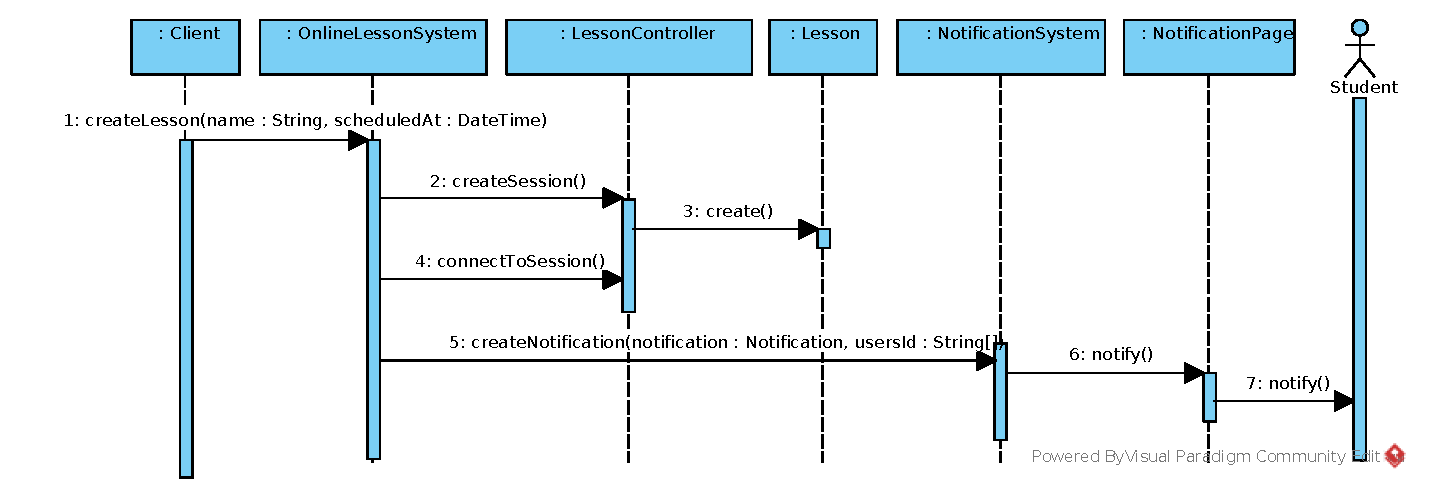
\includegraphics[width=\linewidth]{ss_OnlineLessonSystem_createLesson.eps}
    \caption{Tạo bài giảng online mới}
    \label{ss_ols_cl}
\end{figure}

\begin{figure}[H]
    \centering
    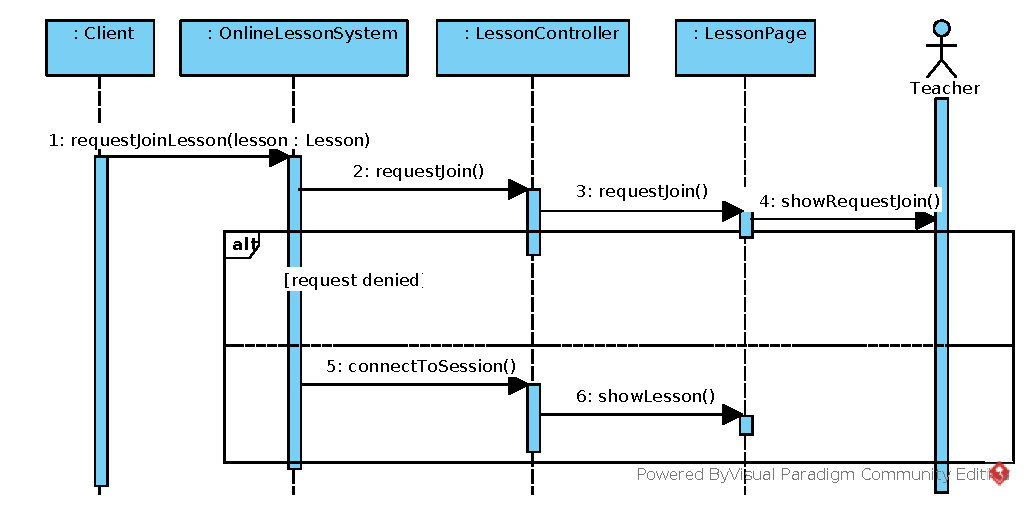
\includegraphics[width=\linewidth]{ss_OnlineLessonSystem_joinLesson.eps}
    \caption{Yêu cầu tham gia bài học online}
    \label{ss_ols_rjl}
\end{figure}

\begin{figure}[H]
    \centering
    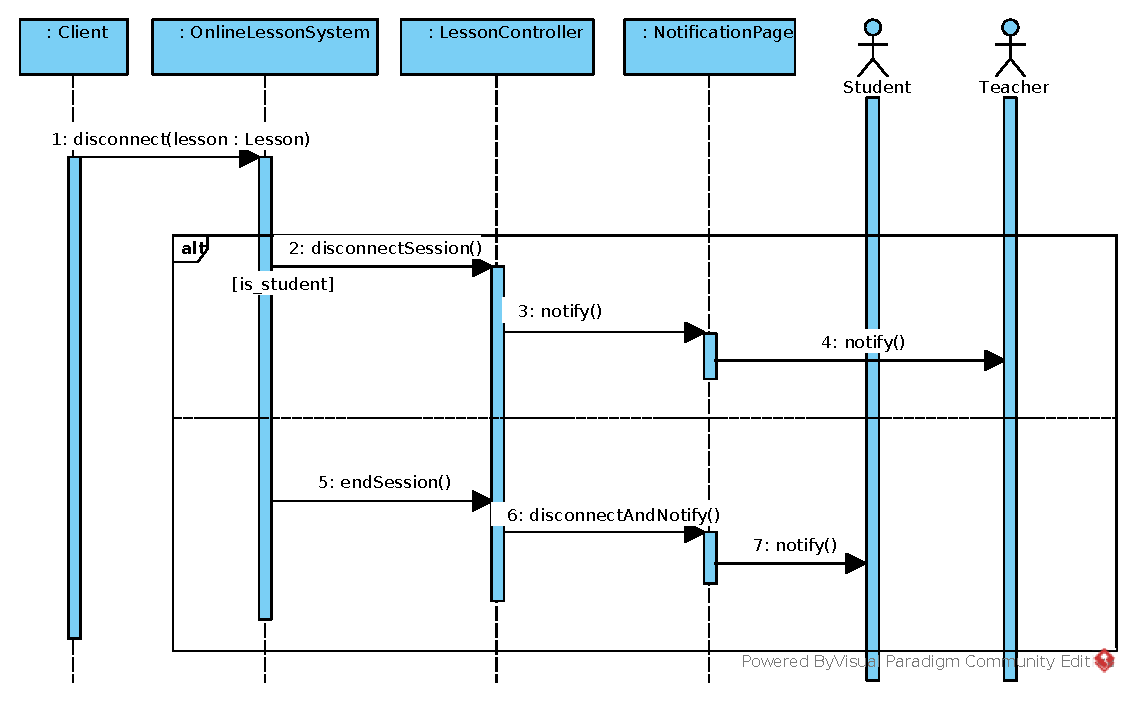
\includegraphics[width=\linewidth]{ss_OnlineLessonSystem_disconnect.eps}
    \caption{Ngắt kết nối với bài học}
    \label{ss_ols_d}
\end{figure}
\subsubsection{Biểu đồ các lớp liên quan}
\begin{figure}[H]
    \centering
    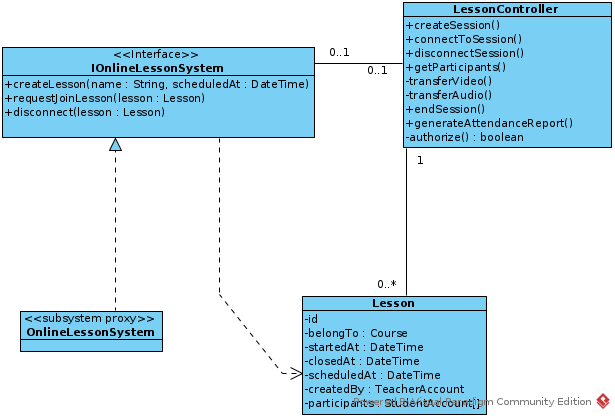
\includegraphics[width=\linewidth]{ss_OnlineLessonSubsystem.png}
    \caption{Biểu đồ các lớp liên quan OnlineLessonSystem}
\label{ss_ols}
\end{figure}
\subsubsection{Biểu đồ lớp phụ thuộc hệ thống con}
\begin{figure}[H]
    \centering
    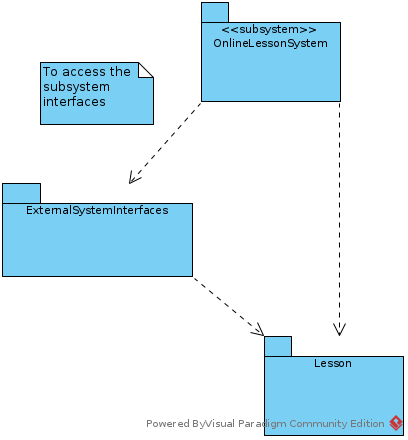
\includegraphics[width=\linewidth]{dp_OnlineLessonSystem.png}
    \caption{Biểu đồ phụ thuộc hệ thống con OnlineLessonSystem}
    \label{dp_ols}
\end{figure}

\subsection{Hệ thống con MessageSystem}
\subsubsection{Hiện thực hóa giao diện}
\begin{figure}[H]
    \centering
    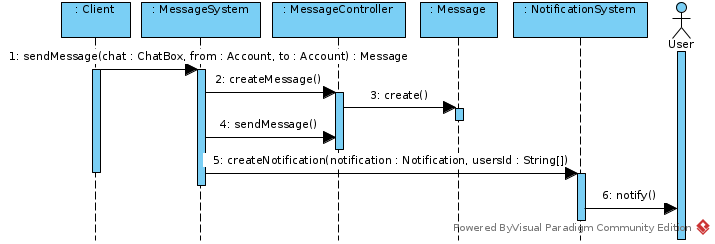
\includegraphics[width=\linewidth]{ss_MessageSystem_sendMessage.png}
    \caption{Gửi tin nhắn}
    \label{ss_ms_sm}
\end{figure}
\subsubsection{Biểu đồ các lớp liên quan}
\begin{figure}[H]
    \centering
    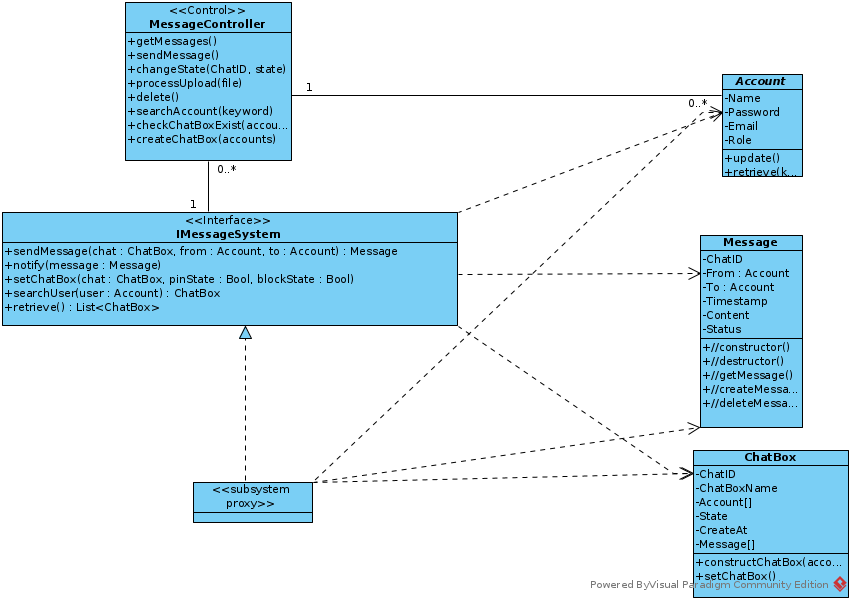
\includegraphics[width=\linewidth]{ss_MessageSystem.png}
    \caption{Biểu đồ các lớp liên quan MessageSystem}
    \label{ss_ms}
\end{figure}
\subsubsection{Biểu đồ lớp phụ thuộc hệ thống con}
\begin{figure}[H]
    \centering
    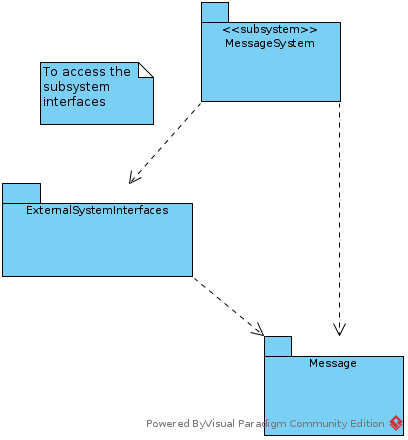
\includegraphics[width=\linewidth]{dp_MessageSystem.png}
    \caption{Biểu đồ lớp phụ thuộc hệ thống con MessageSystem}
    \label{<label>}
\end{figure}

\subsection{Hệ thống con BlogSystem}
\subsubsection{Hiện thực hóa giao diện}
\begin{figure}[H]
    \centering
    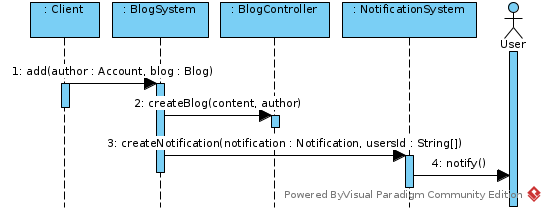
\includegraphics[width=\linewidth]{ss_BlogSystem_add.png}
    \caption{Tạo blog mới}
    \label{ss_bs_a}
\end{figure}
\subsubsection{Biểu đồ các lớp liên quan}
\begin{figure}[H]
    \centering
    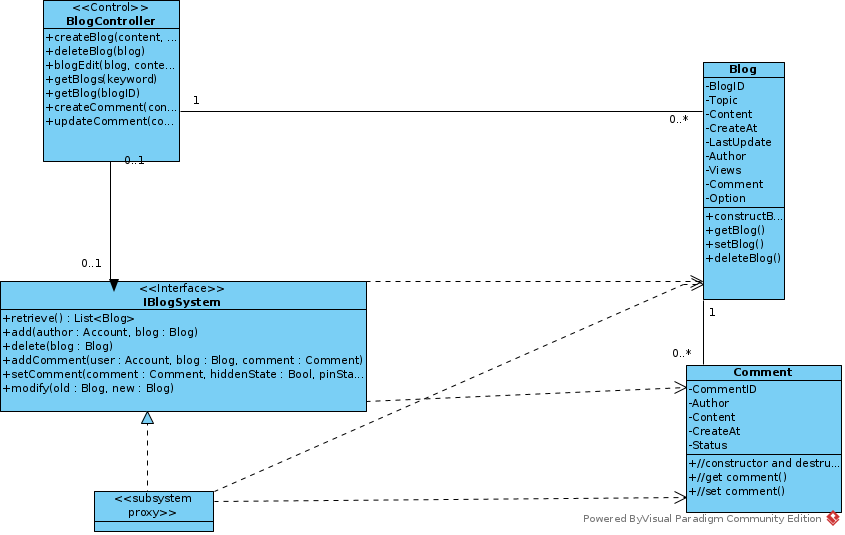
\includegraphics[width=\linewidth]{ss_BlogSystem.png}
    \caption{Biểu đồ các lớp liên quan BlogSystem}
    \label{ss_bs}
\end{figure}
\subsubsection{Biểu đồ lớp phụ thuộc hệ thống con}
\begin{figure}[H]
    \centering
    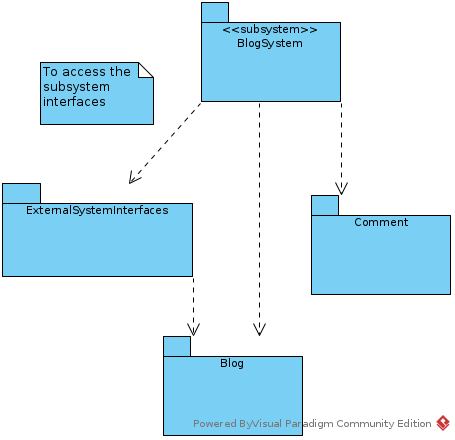
\includegraphics[width=\linewidth]{dp_BlogSystem.png}
    \caption{Biểu đồ lớp phụ thuộc hệ thống con BlogSystem}
    \label{dp_bs}
\end{figure}

\subsection{Hệ thống con NotificationSystem}
\subsubsection{Hiện thực hóa giao diện}
\begin{figure}[H]
    \centering
    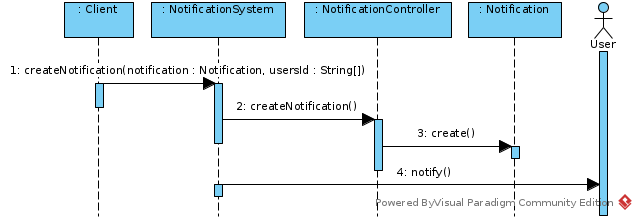
\includegraphics[width=\linewidth]{ss_NotificationSystem_createNotification.png}
    \caption{Tạo thông báo mới}
    \label{ss_ns_cn}
\end{figure}
\subsubsection{Biểu đồ các lớp liên quan}
\begin{figure}[H]
    \centering
    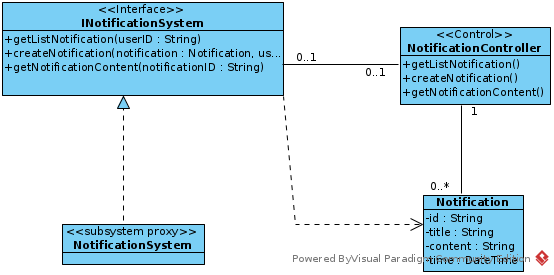
\includegraphics[width=\linewidth]{ss_NotificationSystem.png}
    \caption{Biểu đồ các lớp liên quan NotificationSystem}
    \label{ss_ns}
\end{figure}
\subsubsection{Biểu đồ lớp phụ thuộc hệ thống con}
\begin{figure}[H]
    \centering
    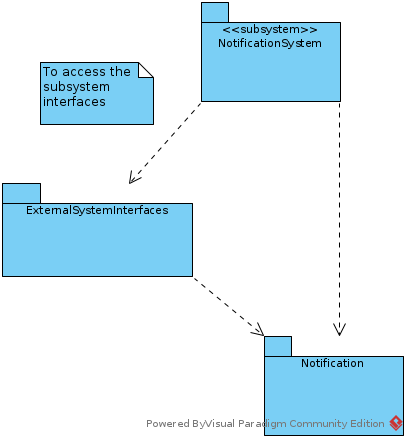
\includegraphics[width=\linewidth]{dp_NotificationSystem.png}
    \caption{Biểu đồ lớp phụ thuộc hệ thống con NotificationSystem}
    \label{dp_ns}
\end{figure}

\subsection{Hệ thống con AssignmentSystem}
\subsubsection{Hiện thực hóa giao diện}
\begin{figure}[H]
    \centering
    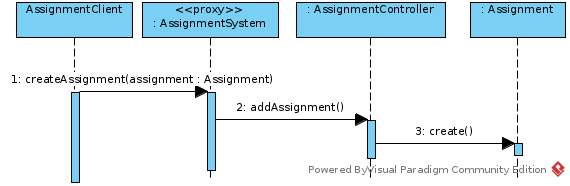
\includegraphics[width=\linewidth]{ss_AssignmentSystem_createAssignment.png}
    \caption{Tạo bài tập mới}
    \label{ss_as_ca}
\end{figure}

\begin{figure}[H]
    \centering
    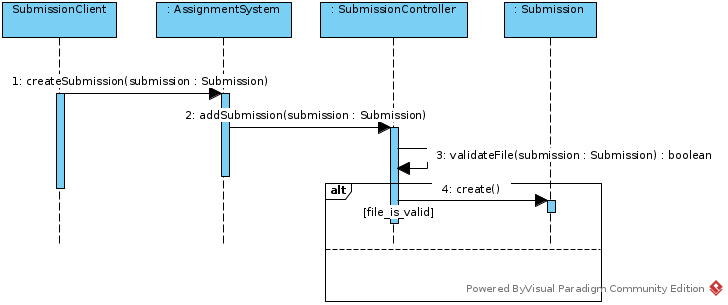
\includegraphics[width=\linewidth]{ss_AssignmentSystem_createSubmission.png}
    \caption{Tạo bài nộp mới}
    \label{ss_as_cs}
\end{figure}

\begin{figure}[H]
    \centering
    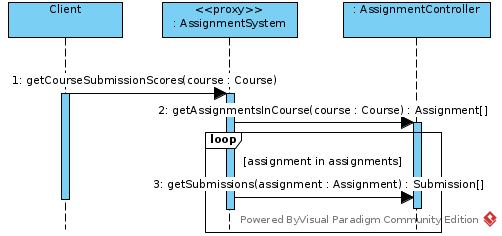
\includegraphics[width=\linewidth]{ss_AssignmentSystem_getCourseSubmissionScores.png}
    \caption{Lấy điểm bài nộp trong khóa học}
    \label{ss_as_gcss}
\end{figure}

\begin{figure}[H]
    \centering
    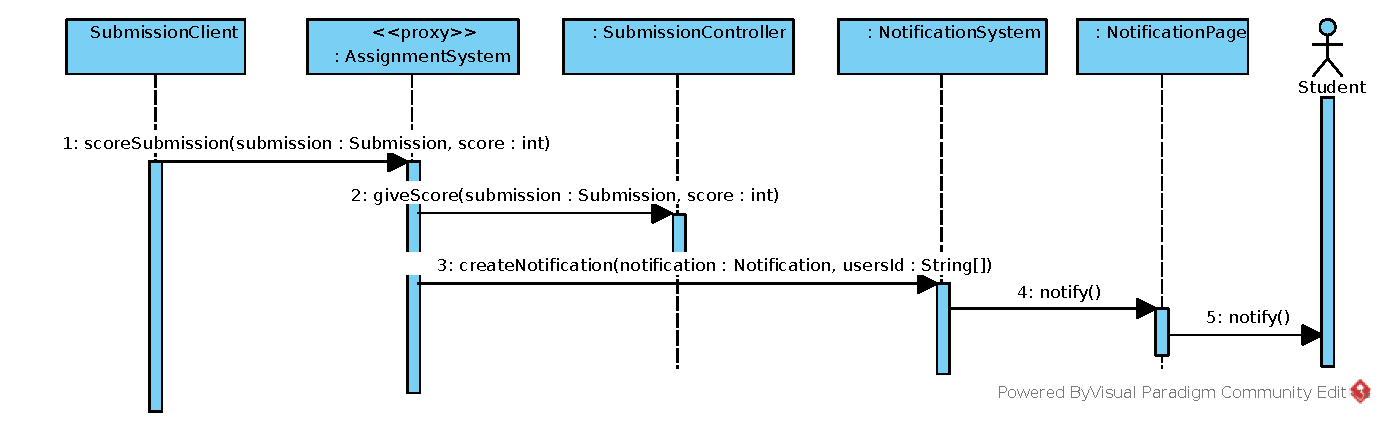
\includegraphics[width=\linewidth]{ss_AssignmentSystem_scoreSubmission.eps}
    \caption{Chấm điểm bài tập}
    \label{ss_as_ss}
\end{figure}
\subsubsection{Biểu đồ các lớp liên quan}
\begin{figure}[H]
    \centering
    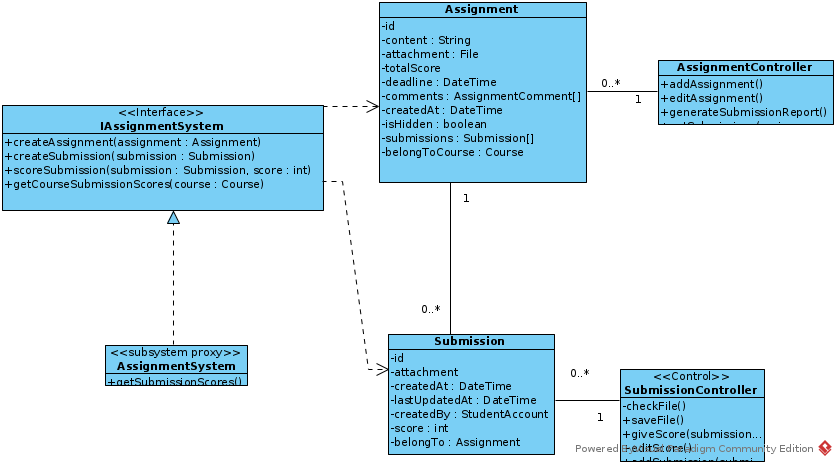
\includegraphics[width=\linewidth]{ss_AssignmentSystem.png}
    \caption{Biểu đồ các lớp liên quan AssignmentSystem}
    \label{ss_as}
\end{figure}
\subsubsection{Biểu đồ lớp phụ thuộc hệ thống con}
\begin{figure}[H]
    \centering
    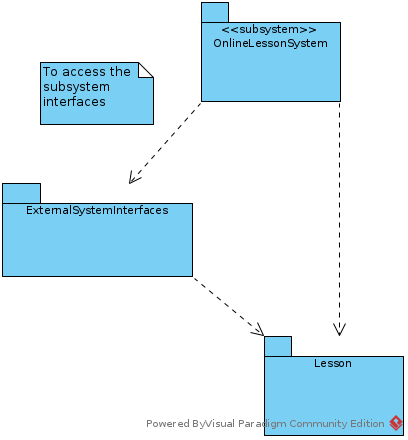
\includegraphics[width=\linewidth]{dp_assignment_system.png}
    \caption{Biểu đồ lớp phụ thuộc hệ thống con AssignmentSystem}
    \label{dp_as}
\end{figure}

\subsection{Hệ thống con AuthenticationSystem}
\subsubsection{Hiện thực hóa giao diện}
\begin{figure}[H]
    \centering
    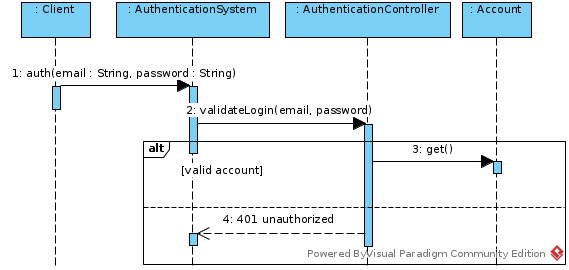
\includegraphics[width=\linewidth]{ss_AuthenticationSystem_auth.png}
    \caption{Xác thực người dùng}
    \label{ss_aus_a}
\end{figure}
\subsubsection{Biểu đồ các lớp liên quan}
\begin{figure}[H]
    \centering
    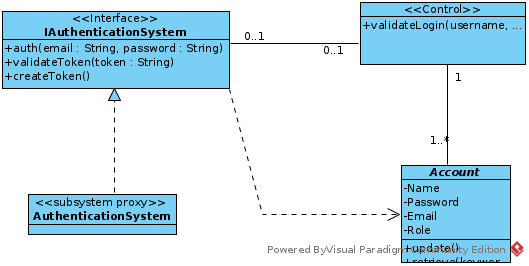
\includegraphics[width=\linewidth]{ss_AuthenticationSystem.png}
    \caption{Biểu đồ các lớp liên quan AuthenticationSystem}
    \label{ss_aus}
\end{figure}
\subsubsection{Biểu đồ lớp phụ thuộc hệ thống con}
\begin{figure}[H]
    \centering
    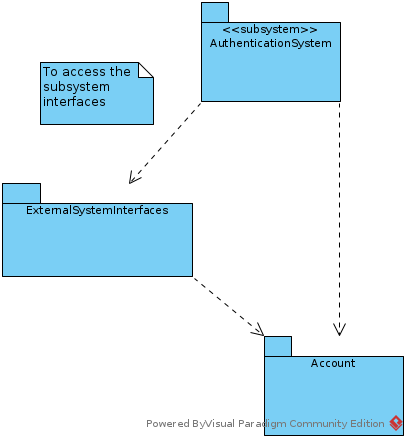
\includegraphics[width=\linewidth]{dp_AuthenticationSystem.png}
    \caption{Biểu đồ lớp phụ thuộc hệ thống con}
    \label{dp_aus}
\end{figure}

\end{document}